\section{Application}\label{sec:resultApp}
This section presents the resulting implementation of the Apple iOS application.

\bigskip

In \Cref{subfig:machinesList} the result of the application screen to set a position and show the corresponding machines is being presented.
\Cref{sec:implAppSetPos} describes technical details how machines is being presented when a position is set.

\bigskip

\Cref{subfig:machineDetails} present the application screen to look at the details for a machine.
This screen is meant to present the documents and real-time process data for a selected machine, which is not being done in this thesis. 

\bigskip

\Cref{subfig:nearbyBeacons} present a screen that shows all nearby beacons with its value that the application can read.

\bigskip

In \Cref{subfig:existingGroups} all created groups is being presented.
From this screen the details about a group can be viewed, presented in \Cref{subfig:groupDetails}.
Another feature is to create new groups within the application, which is being presented in \Cref{subfig:newGroup}.
How the new group feature is implemented is being described in \cref{sec:implAppNewGroup}.

\begin{figure}[H]
	\centering
	\begin{subfigure}[t]{0.3\textwidth}
		\centering	
		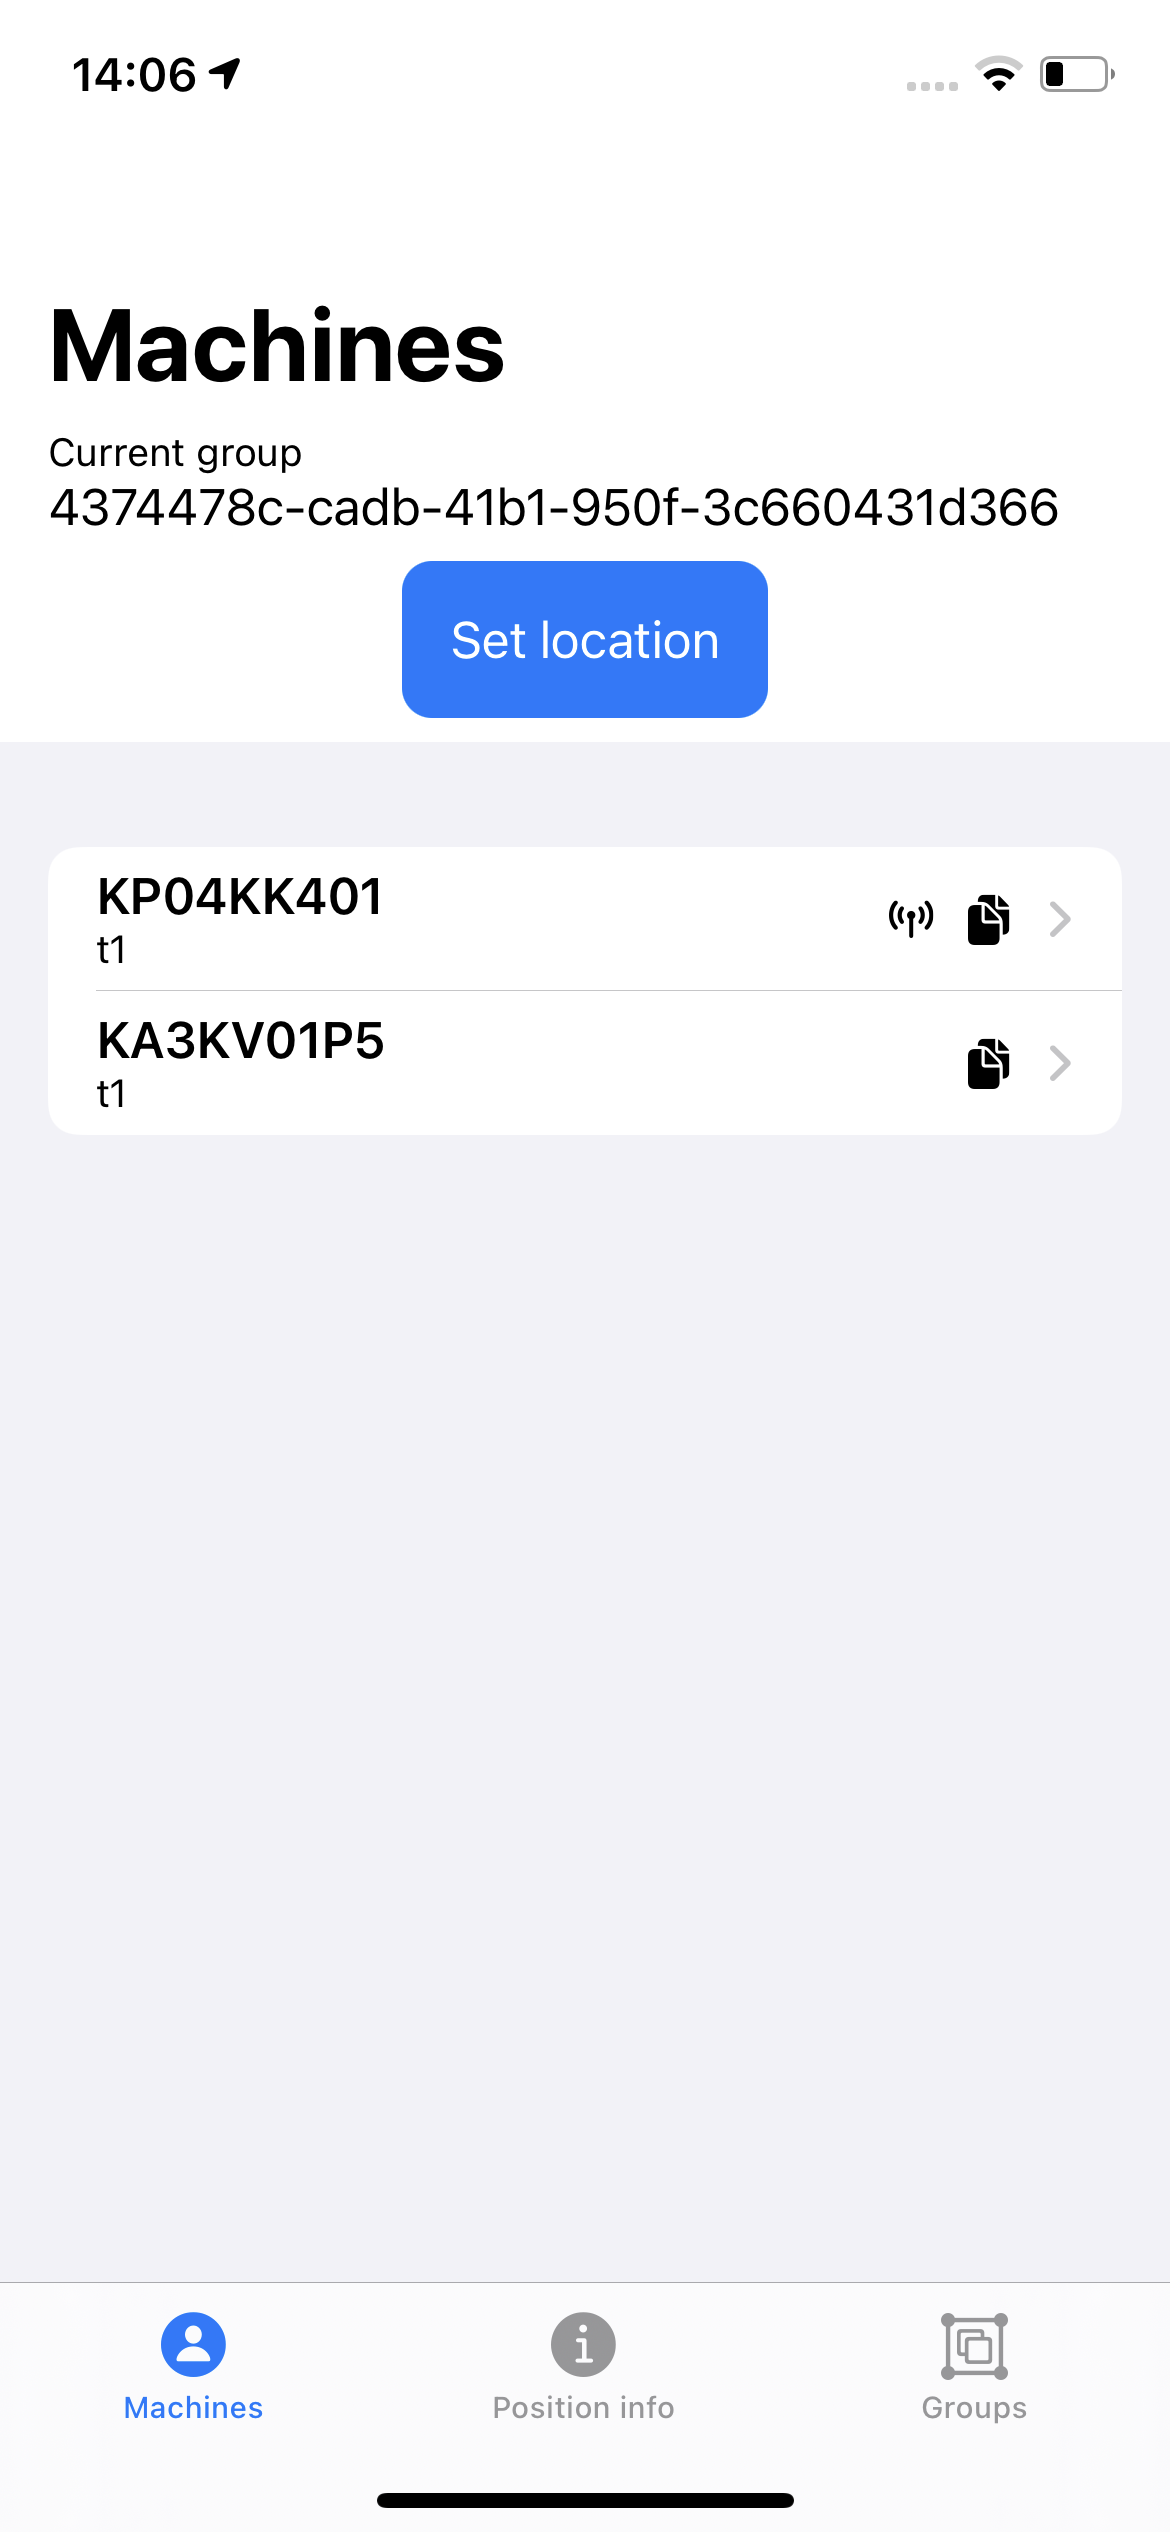
\includegraphics[width=.9\textwidth]{appScreens/machinesGroup}
		\caption{Machines list}
		\label{subfig:machinesList}
	\end{subfigure}%
	\begin{subfigure}[t]{0.3\textwidth}
		\centering	
		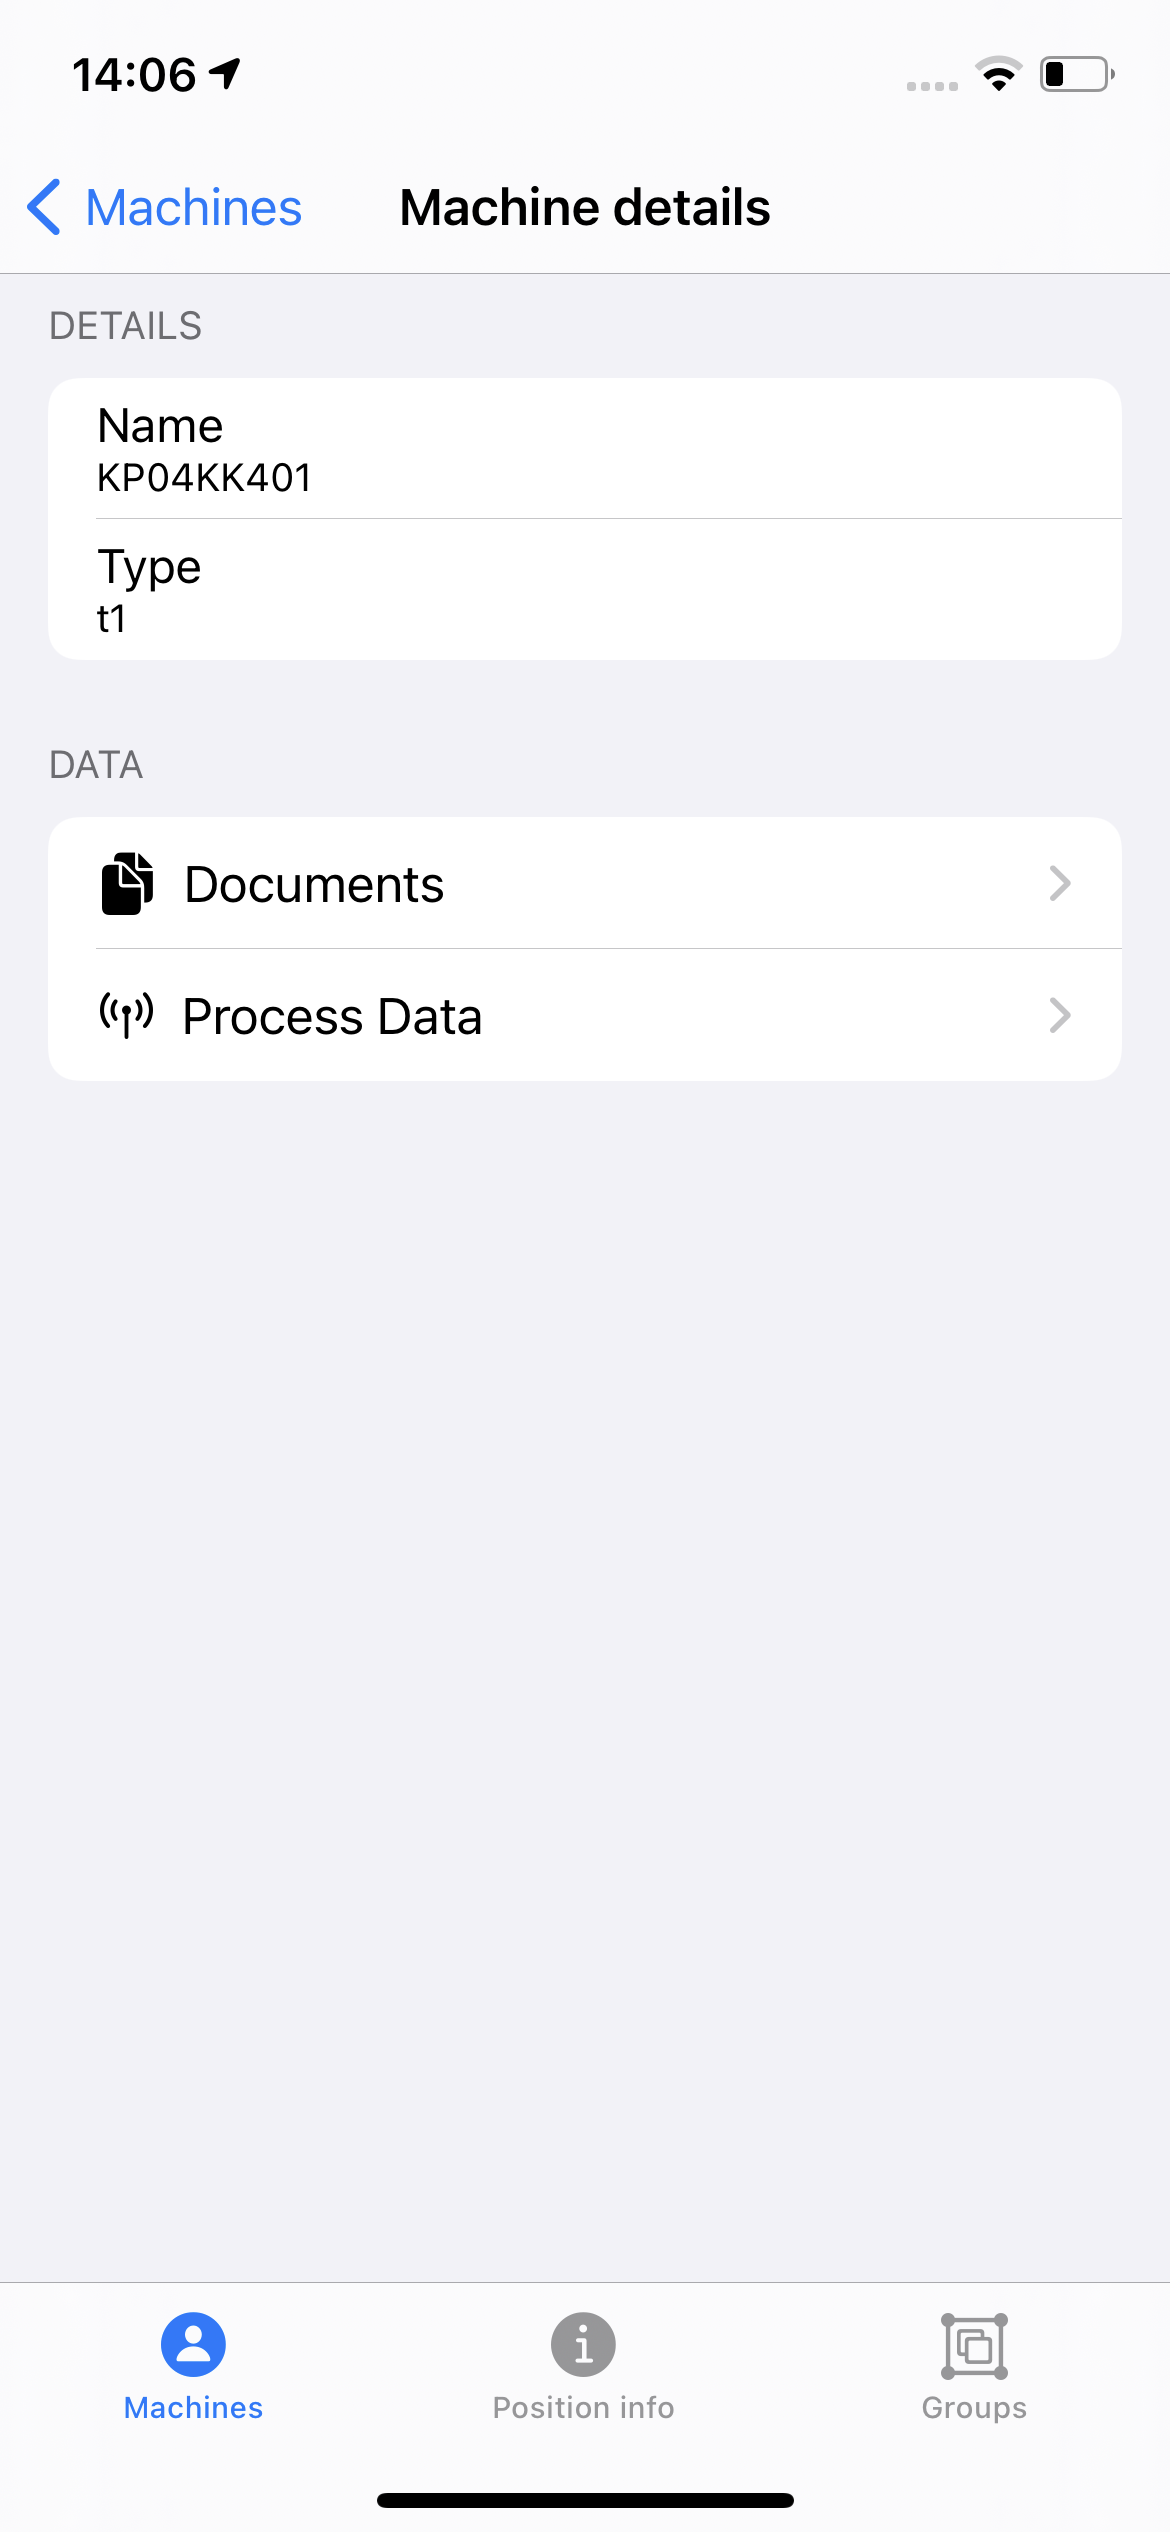
\includegraphics[width=.9\textwidth]{appScreens/machineDetails}
		\caption{Machine details}
		\label{subfig:machineDetails}
	\end{subfigure}
	\begin{subfigure}[t]{0.3\textwidth}
		\centering	
		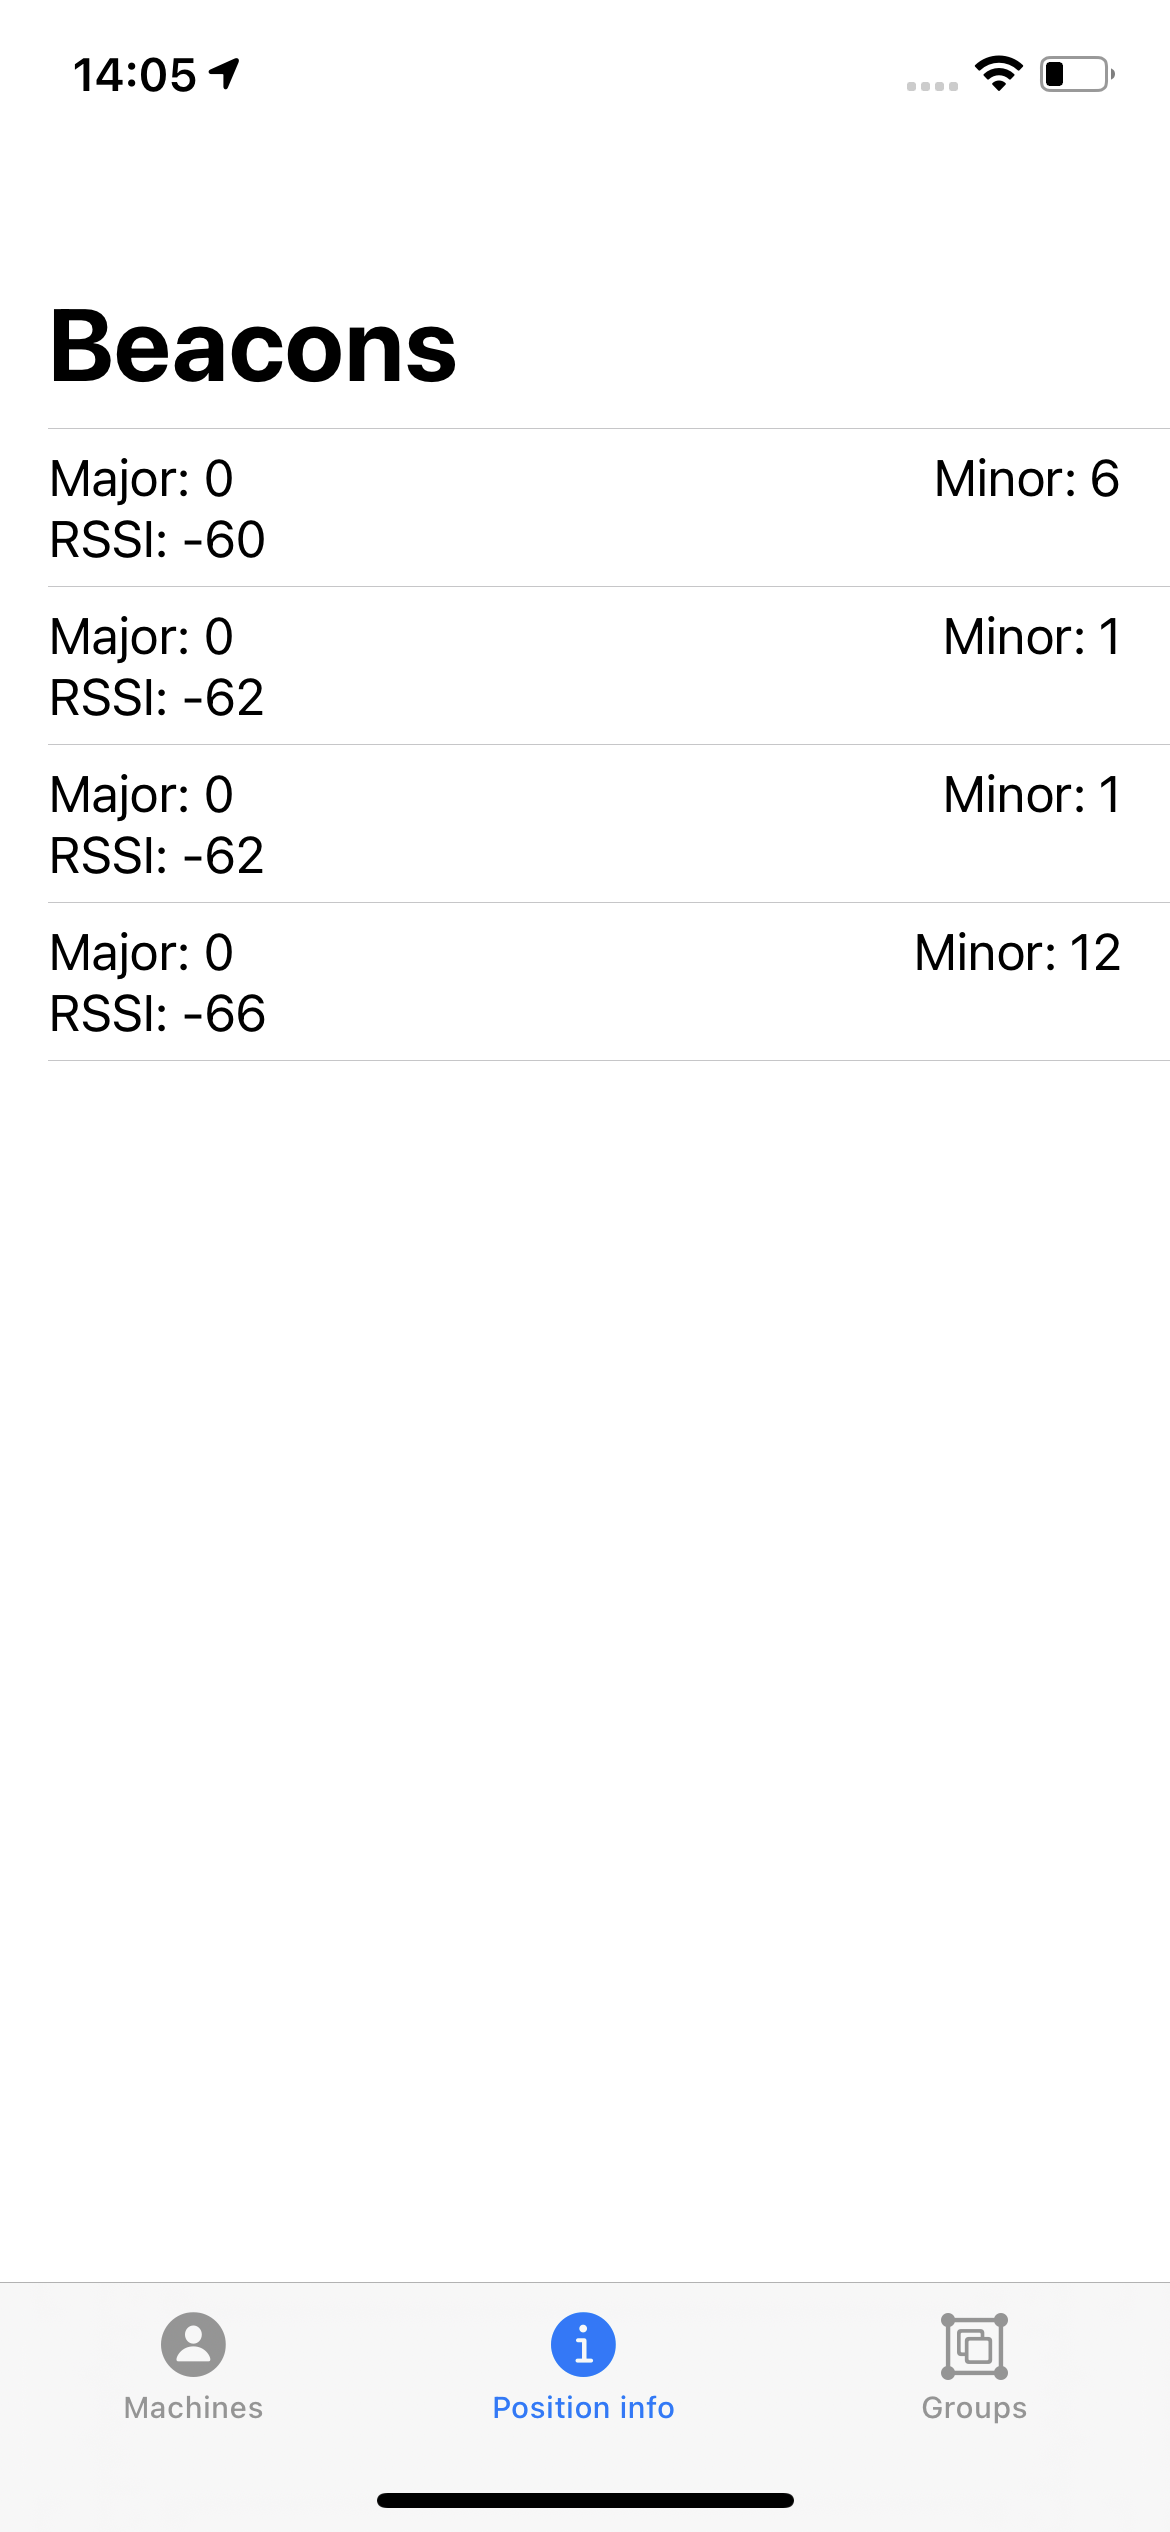
\includegraphics[width=.9\textwidth]{appScreens/beacons}
		\caption{Nearby beacons}
		\label{subfig:nearbyBeacons}
	\end{subfigure}
	\begin{subfigure}[t]{0.3\textwidth}
		\centering	
		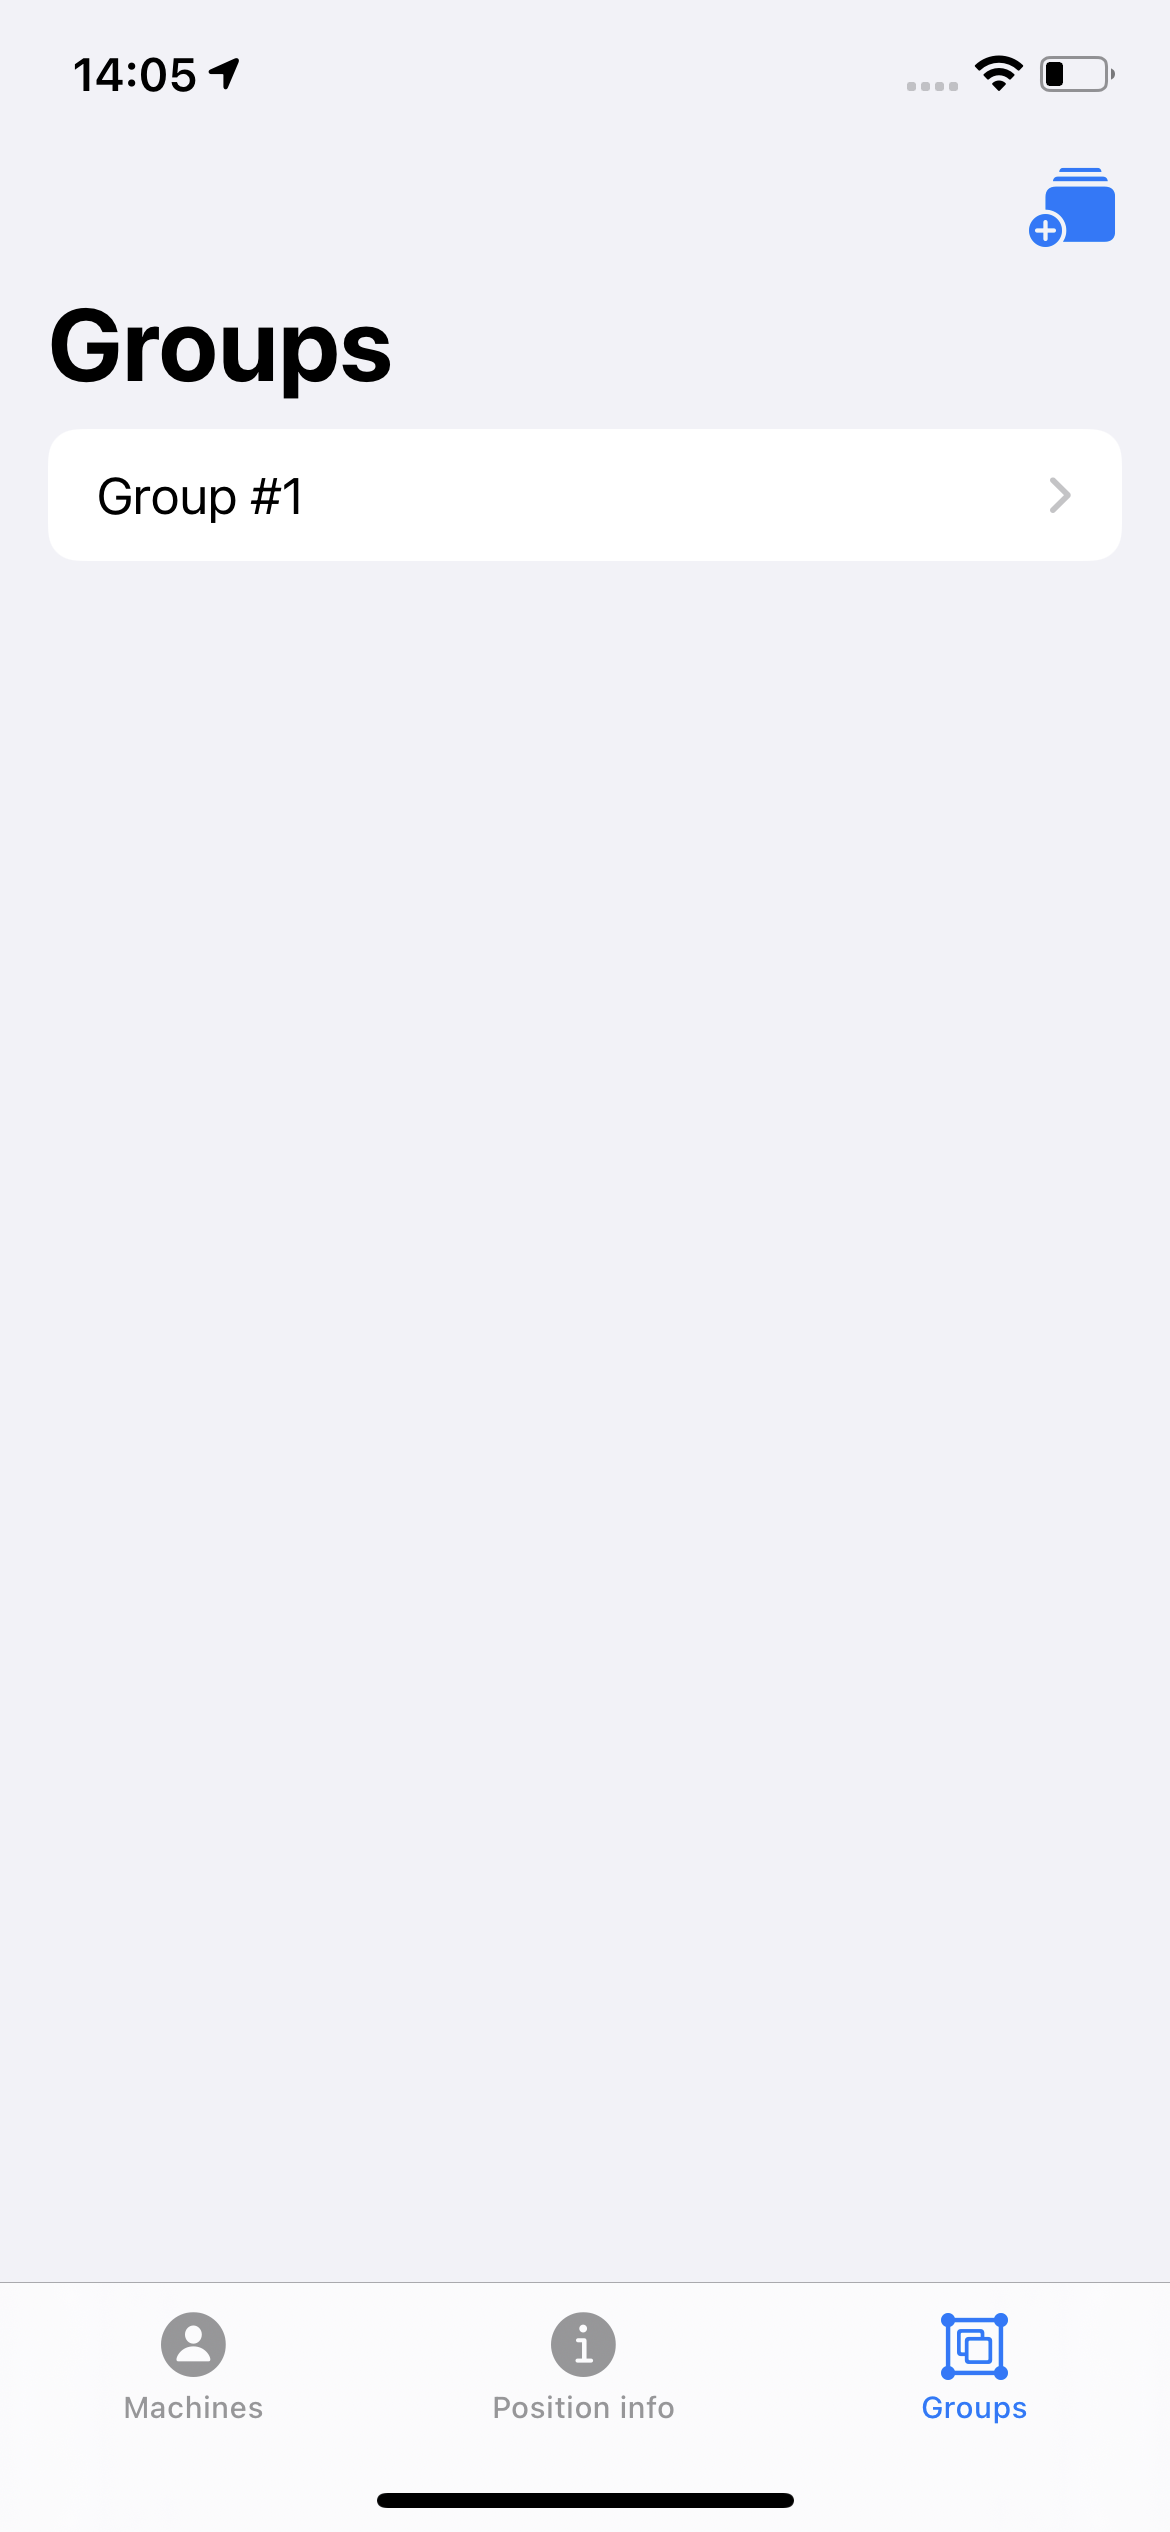
\includegraphics[width=.9\textwidth]{appScreens/groups}
		\caption{Existing groups}
		\label{subfig:existingGroups}
	\end{subfigure}
	\begin{subfigure}[t]{0.3\textwidth}
		\centering	
		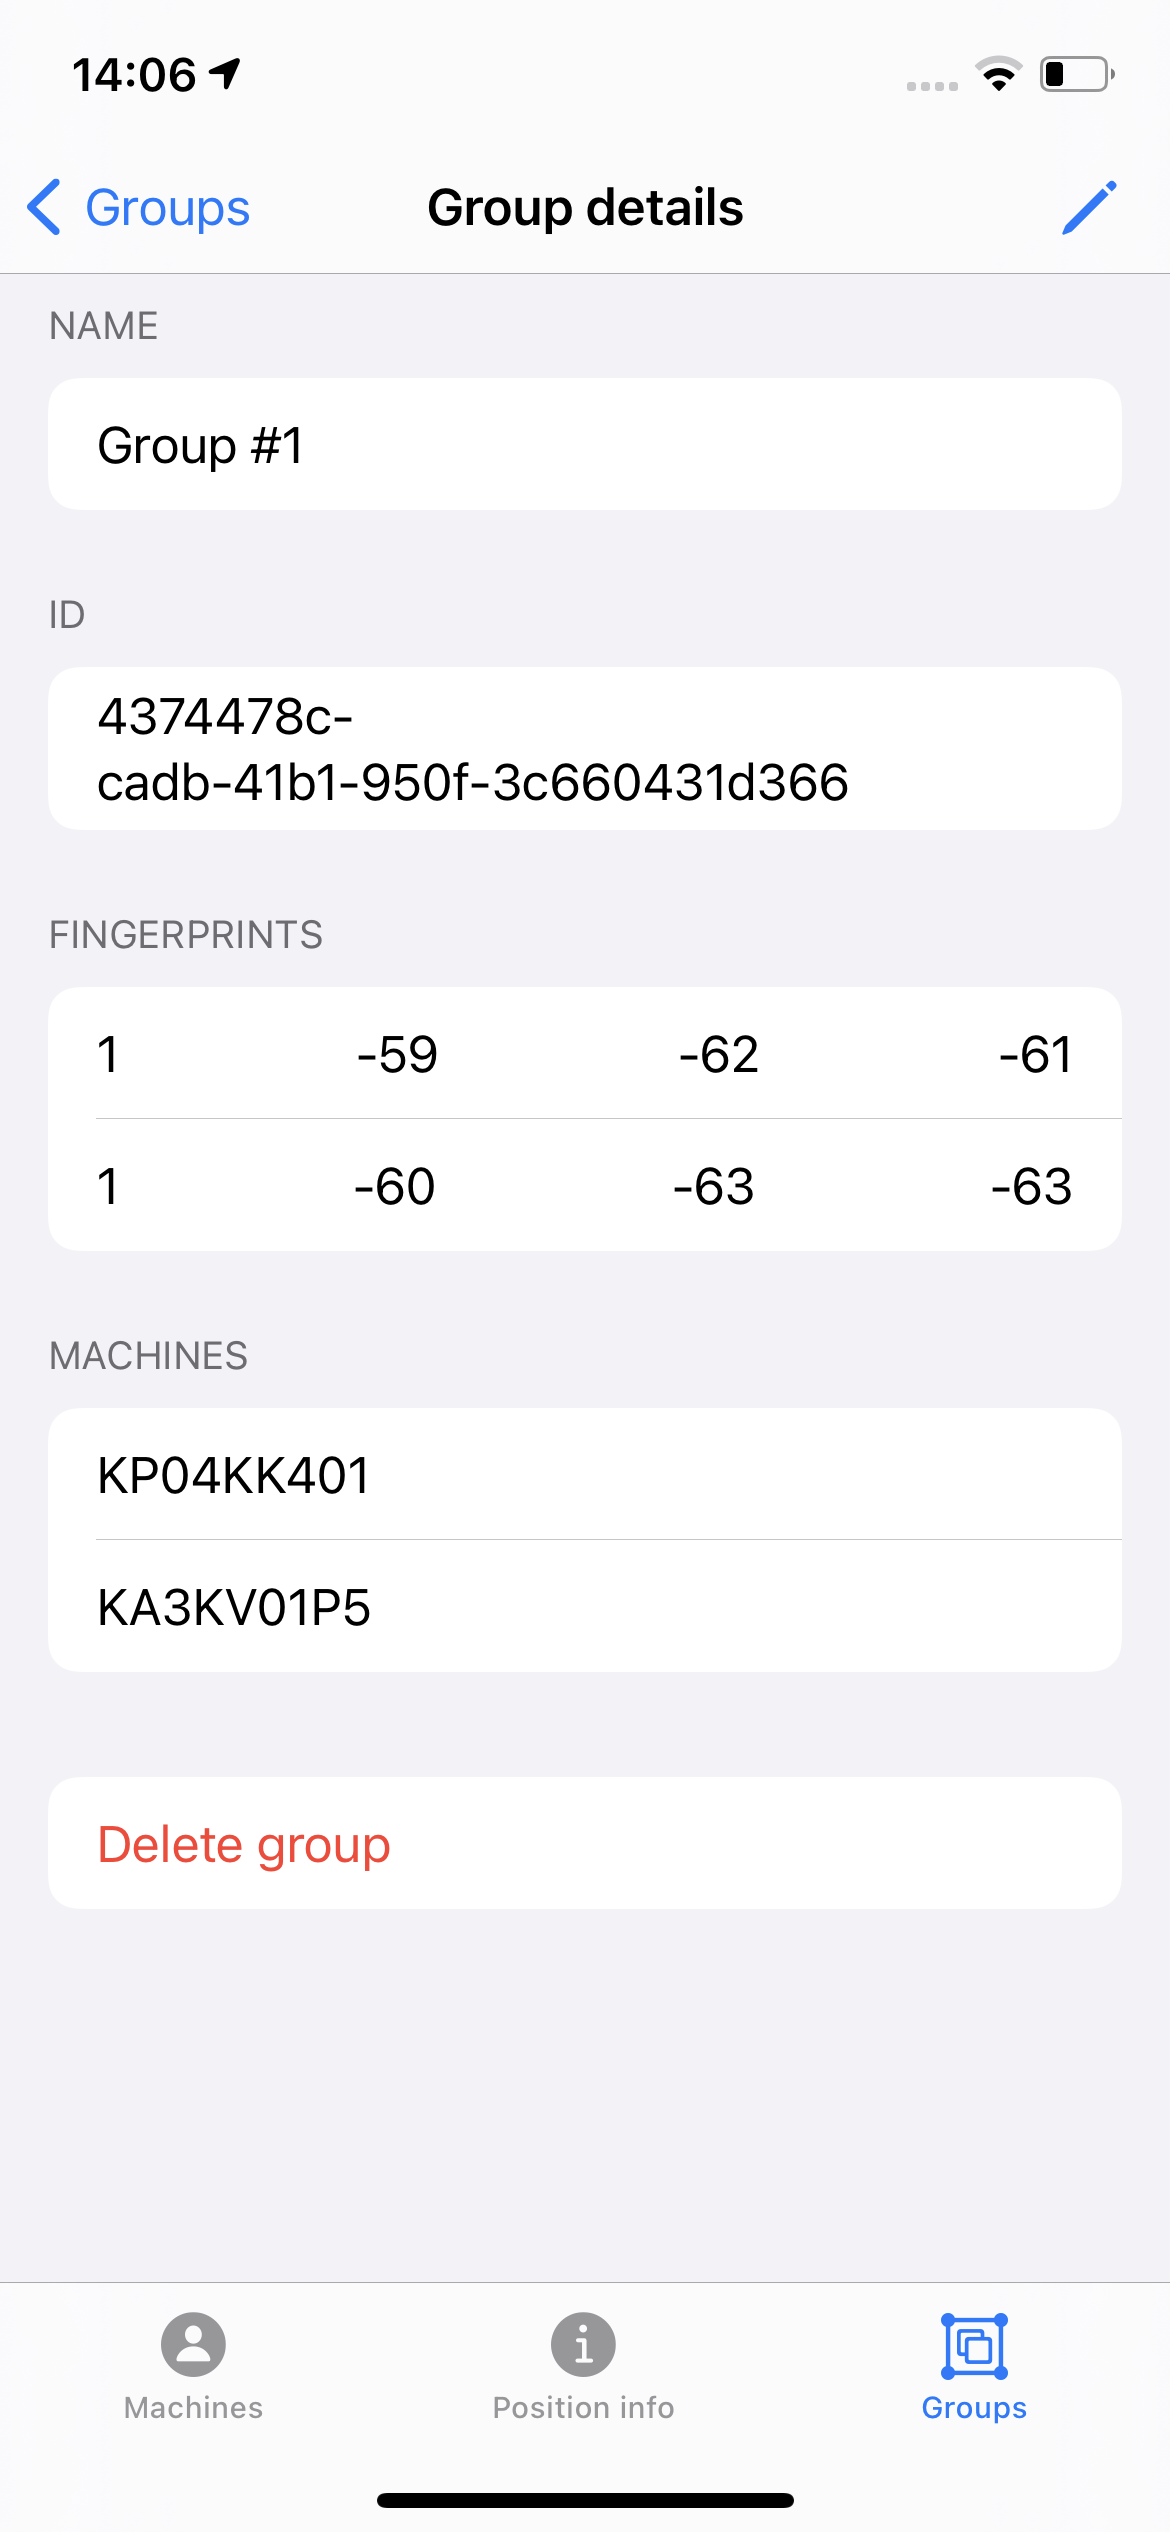
\includegraphics[width=.9\textwidth]{appScreens/groupDetails}
		\caption{Group details}
		\label{subfig:groupDetails}
	\end{subfigure}
	\begin{subfigure}[t]{0.3\textwidth}
		\centering	
		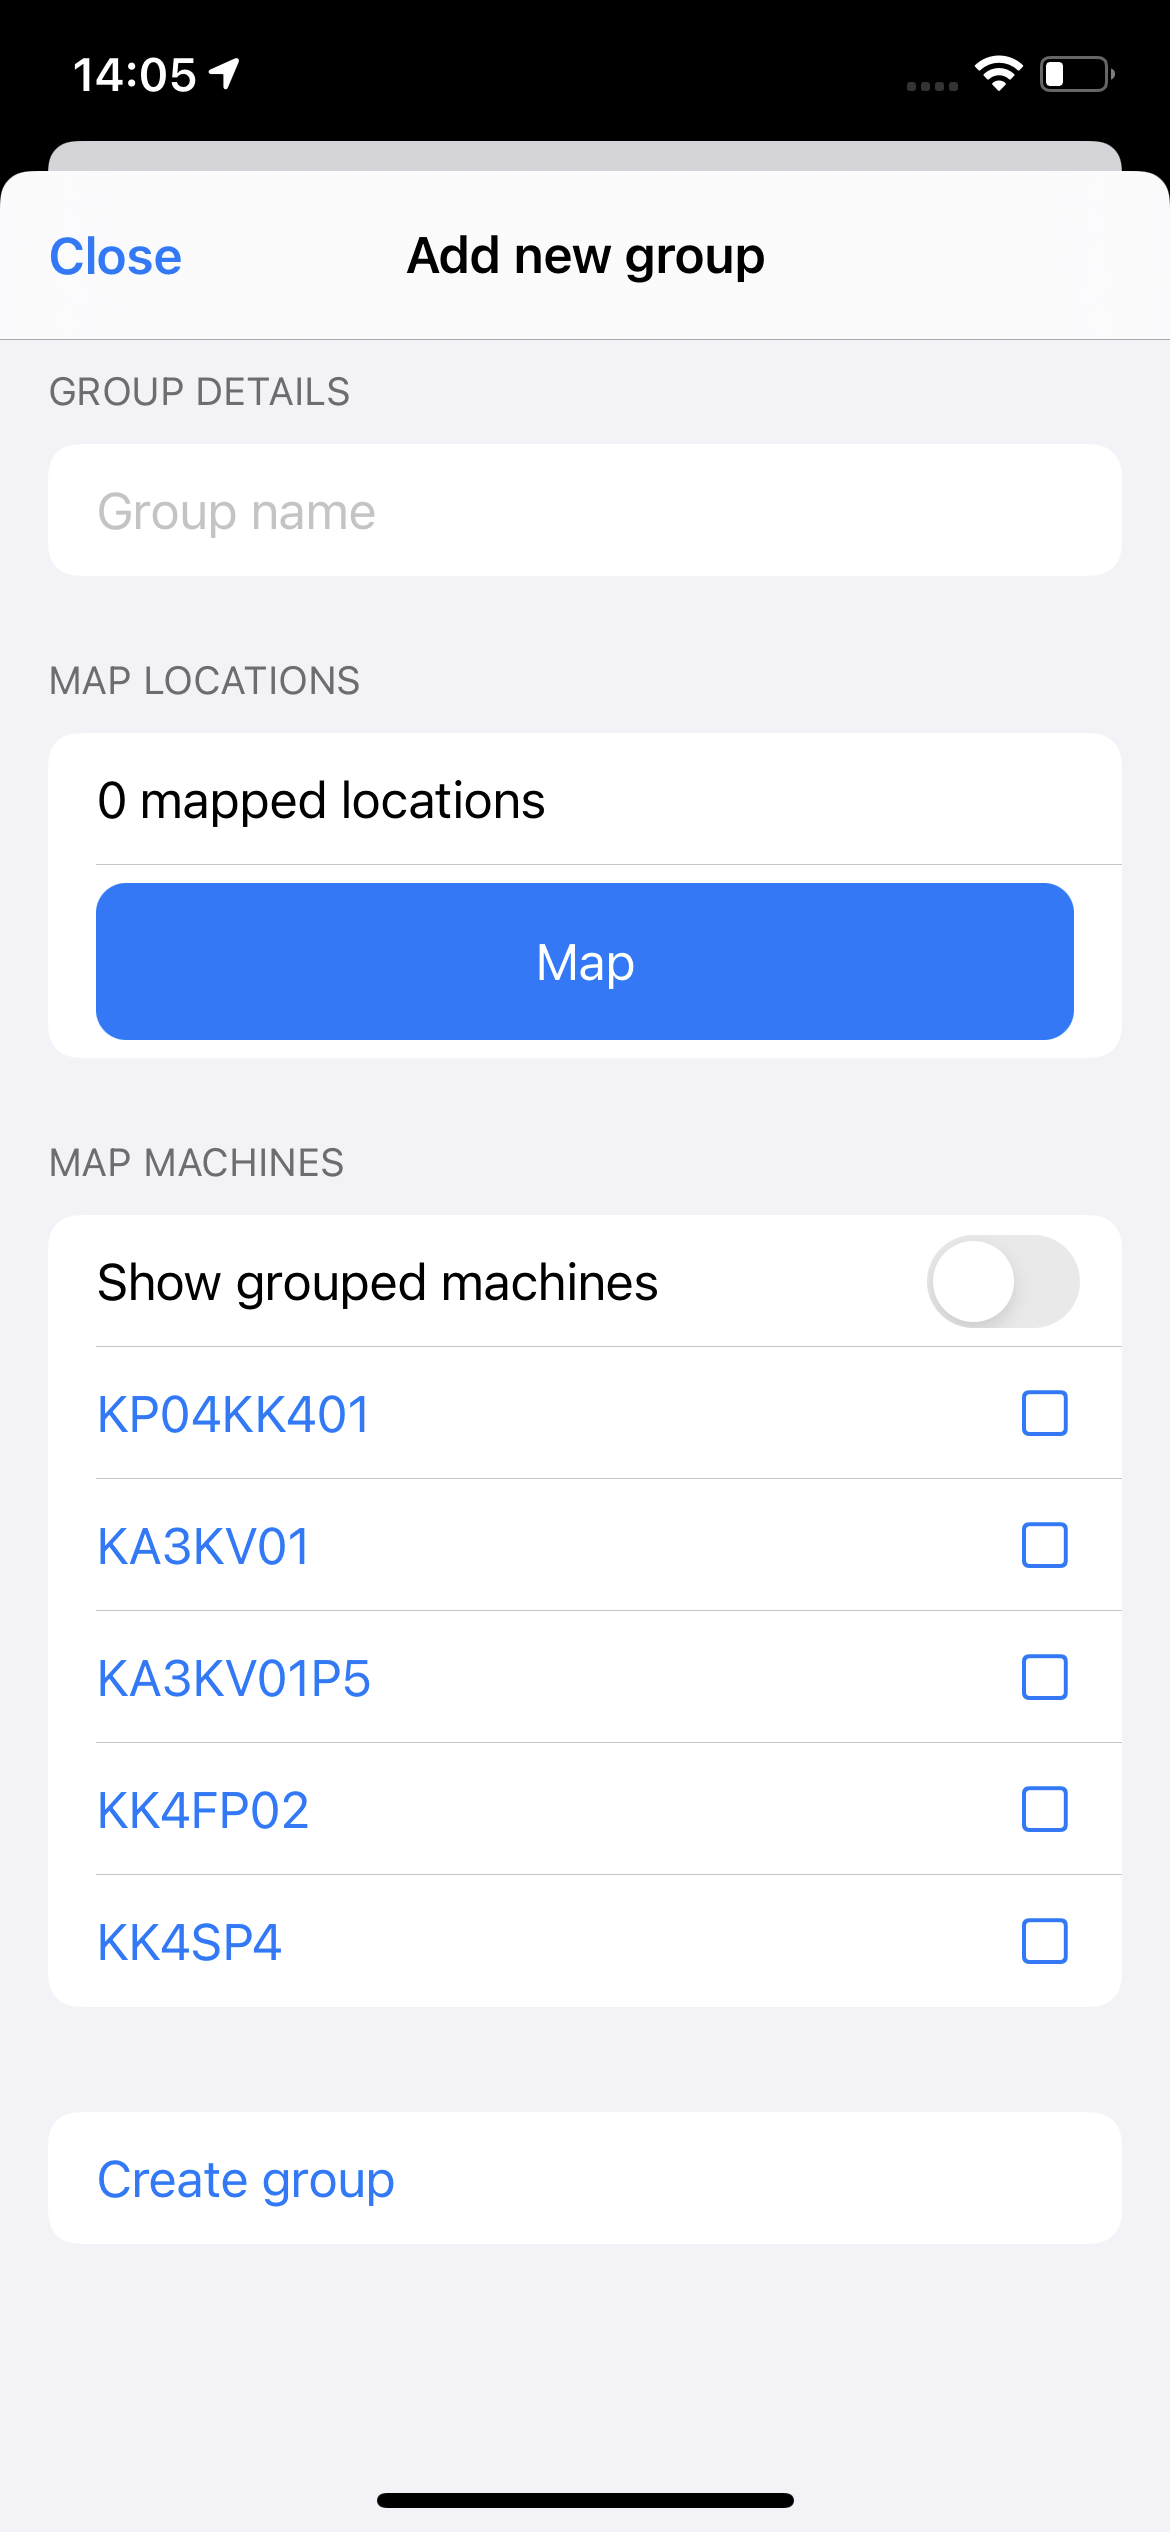
\includegraphics[width=.9\textwidth]{appScreens/newGroup}
		\caption{New group}
		\label{subfig:newGroup}
	\end{subfigure}

	\caption{Application screens}
	\label{fig:appScreens}

\end{figure}

